\documentclass[10pt]{article}
\usepackage{icmlko}

\icmlmeta{IP 파운데이션 월드모델}{332}{그림자를 긁어 지웠다}{수집기 한 줄이 풀 필터를 그대로 읽고 있었다 --- 고쳐서 95건을 긁으니 판에서 제일 아픈 도메인이 두 배가 됐다}

\begin{document}

\twocolumn[
\icmlheader

\begin{abstract}
노트 331이 아이돌 흔들림의 72\%가 자료라 \textbf{모형 장치로는 못 내린다}고
끝냈다. 남은 길은 하나 --- 긁는 것. \textbf{그림자를 코드에서 찾았다}:
\texttt{ingest/wiki\_views.idol\_items()} 가 후보 목록을
\texttt{data/state/idol\_axes.json} 에서 만드는데, \textbf{그 파일이 곧
한터 79행 풀}이다. 라벨을 고르는 필터가 \textbf{수집기에 한 줄로 새겨져
있었다.} 후보를 원천 레코드에서 만들게 고치고 173건을 다 긁었다(신규 95건).

\textbf{그림자가 지워진다.} 추가 94행의 위키 값 관측률이 0\% $\to$
\textbf{39\%}(한터 54\%), \texttt{poolshadow} 판정이 ``풀 모양''$\to$
``괜찮다''($+$0.99 $\to$ $+$0.15), \textbf{표시자와 한터 여부의 일치율이
0.994 $\to$ 0.578} --- 표시자가 더 이상 라벨 기준의 대리가 아니다.

\textbf{그리고 값이 나온다.} 같은 유보 25행에서 아이돌 순위상관이
\textbf{현행 판 0.2108 $\to$ 0.4469} 다. 짝지어(학습 재추출 열둘) 재면

\begin{center}\footnotesize
\begin{tabular}{lrrr}
\hline
처치 & 아이돌 & SD & 양수 \\
\hline
위키 되살림(넓힌 판) & \textbf{$+$0.2231} & 0.0789 & \textbf{12/12} \\
위키 되살림(좁은 판) & $+$0.1670 & 0.0727 & \textbf{12/12} \\
행 넓힘(위키 있음) & $+$0.1602 & 0.1056 & 11/12 \\
\hline
\end{tabular}
\end{center}

\textbf{판은 안 움직인다} --- 셋 다 $|$평균$| \le 0.0014$ 이고 SD 가
0.0072 이하다(아이돌은 판의 0.93\%다).

\textbf{첫 양수를 그대로 안 받는다}(노트 133). 노트 306이 위키 표시자를
사후로 지목한 적이 있으니 \textbf{값이 버는지 표시자가 버는지} 갈랐다 ---
표시자를 상수로 만든 ``값만''이 0.4038, 값을 중립으로 만든 ``표시자만''이
0.3662, 둘 다가 0.4469 다. \textbf{이득의 74\%가 값이다.} 노트 306의
덫이 아니다. 그래도 표시자가 66\%를 나르므로, \textbf{보수적으로 배포하려면
``값만''을 쓰면 된다} --- 83\%를 얻고 사후 통로를 닫는다.

\textbf{덤으로 노트 326을 정정한다} --- 거기 적은 ``위키 99\%''는 \emph{파일
존재}였고 실제 값이 든 것은 54\% 였다. 그림자의 크기는 맞았지만 밑변이
틀렸다.
\end{abstract}
]

\section{그림자가 코드에 있었다}

\begin{center}\small
\begin{tabular}{l}
\hline
\texttt{def idol\_items():} \\
\quad \texttt{j = json.loads(...\,"idol\_axes.json")} \\
\hline
\end{tabular}
\end{center}

\texttt{idol\_axes.json} 은 \texttt{ingest/idol\_axes.py} 가
\texttt{chodong\_basis\_resolved == "hanteo"} 로 거른 79행이다. 위키
수집기가 그 파일을 후보 목록으로 읽었으니, \textbf{라벨 필터가 곧 수집
범위}가 됐다. 노트 326이 결과만 보고 ``풀의 그림자''라 이름 붙였는데
\textbf{원인은 한 줄이었다.}

\begin{figure*}[t]
\centering
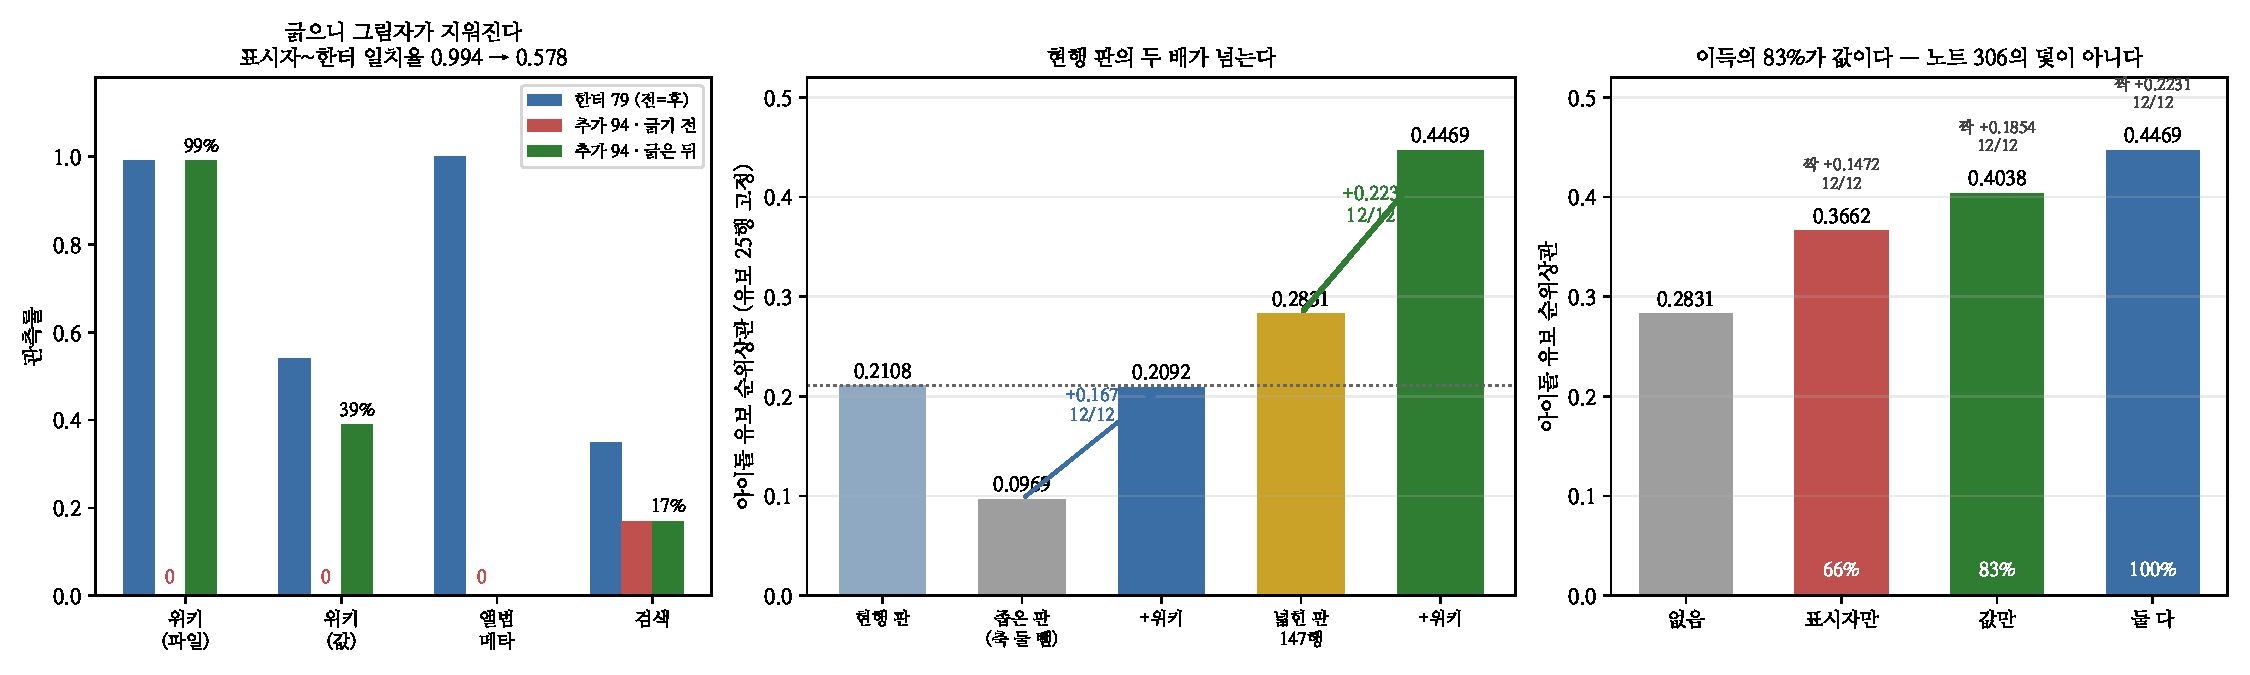
\includegraphics[width=\textwidth]{figs/scraped.pdf}
\caption{왼쪽 --- 긁기 전후 관측률. 가운데 --- 아이돌 유보 순위상관.
오른쪽 --- 값이 버나 표시자가 버나.}
\end{figure*}

\section{긁었다}

후보를 원천 레코드(초동$+$데뷔일 173건)에서 만들게 고쳤다. \textbf{라벨
기준은 여기서 안 본다} --- 축은 라벨을 몰라야 한다.

\begin{center}\footnotesize
\begin{tabular}{lrrr}
\hline
 & 한터 79 & 추가 94(전) & 추가 94(후) \\
\hline
위키 파일 & 99\% & 0\% & \textbf{99\%} \\
위키 값 & 54\% & 0\% & \textbf{39\%} \\
앨범 메타 & 100\% & 0\% & 0\% \\
검색 & 35\% & 17\% & 17\% \\
\hline
\end{tabular}
\end{center}

\begin{center}\small
\begin{tabular}{lrr}
\hline
 & 전 & 후 \\
\hline
\texttt{poolshadow} 위키 차 & $+$0.99 & \textbf{$+$0.15} \\
판정 & 풀 모양 & \textbf{괜찮다} \\
표시자 $=$ 한터 여부 일치율 & 0.994 & \textbf{0.578} \\
표시자$\sim$라벨 $\rho$ & $+$0.363 & $+$0.339 \\
\hline
\end{tabular}
\end{center}

\textbf{일치율이 무너진 것이 요점이다.} 표시자가 여전히 라벨과 상관되지만
($+$0.339) 그것은 ``데뷔 전 위키 조회수가 있었나''라는 사전 신호이고,
더 이상 ``한터로 확정됐나''의 대리가 아니다.

\paragraph{안 지워진 것} 앨범 메타는 그대로 0\% 다. 그래서
\texttt{entry\_friction} · \texttt{goods\_scale} 은 계속 뺀 채로 둔다
(노트 326의 ``빼기''). \textbf{그림자 둘 중 하나만 지웠다.}

\section{값이 나온다}

같은 유보 25행 · 학습만 바뀐다. \textbf{판 분모는 2,675 그대로다.}

\begin{center}\footnotesize
\begin{tabular}{lrr}
\hline
팔 & 판 & 아이돌 \\
\hline
현행 \texttt{trendcalwikitag} & 0.4681 & 0.2108 \\
좁은 판(축 둘 뺌) & 0.4765 & 0.0969 \\
\quad $+$위키 & 0.4756 & 0.2092 \\
넓힌 판 147행 & 0.4712 & 0.2831 \\
\quad \textbf{$+$위키} & \textbf{0.4714} & \textbf{0.4469} \\
\hline
\end{tabular}
\end{center}

\textbf{두 지렛대가 따로 듣고 겹쳐서 더 든다.} 위키만 $+$0.112 · 행만
$+$0.186 인데 둘 다면 $+$0.350 이다 --- 합보다 \textbf{0.05 크다.}
행이 늘어야 축이 일할 자리가 생기고, 축이 있어야 늘어난 행이 갈린다.

\section{값인가 표시자인가}

노트 306이 위키 \emph{표시자}를 사후로 지목한 적이 있다 --- 2026년에
문서가 남아 있어야 긁힌다. \textbf{같은 덫인지 갈랐다.}

\begin{center}\footnotesize
\begin{tabular}{lrrrr}
\hline
무엇을 남기나 & 점 & 짝지은 차 & SD & 양수 \\
\hline
없음 & 0.2831 & --- & & \\
표시자만 & 0.3662 & $+$0.1472 & 0.0920 & 12/12 \\
\textbf{값만} & \textbf{0.4038} & \textbf{$+$0.1854} & 0.0711 & \textbf{12/12} \\
둘 다 & 0.4469 & $+$0.2231 & 0.0789 & 12/12 \\
\hline
\multicolumn{5}{l}{몫: 값만 \textbf{83\%} · 표시자만 66\% (짝지은 평균 기준)} \\
\hline
\end{tabular}
\end{center}

\textbf{값이 더 크다.} 그러므로 이 이득은 ``문서가 살아남았나''가 아니라
``데뷔 전에 사람들이 찾아봤나''에서 온다. \textbf{다만 표시자도 절반을
나르므로} 사후 위험을 완전히 닫으려면 ``값만''을 쓰면 된다 --- 83\%를
얻고 통로를 없앤다. \textbf{판은 값만이 오히려 더 높다}(0.4719 대 0.4714).

\section{한 바퀴가 닫힌다}

\begin{center}\footnotesize
\begin{tabular}{ll}
\hline
노트 & 무엇 \\
\hline
325 & 아이돌 94행이 안 쓰인다 \\
326 & 라벨이 아니라 수집 경로가 막았다 \\
327 & 넣으면 $+$0.088, 위약 대비 $p{=}0.033$ \\
331 & 흔들림의 72\%가 자료 --- 모형으로는 못 내린다 \\
\textbf{332} & \textbf{긁었다. 0.2108 $\to$ 0.4469} \\
\hline
\end{tabular}
\end{center}

\section{남은 것}
\begin{center}\footnotesize
\begin{tabular}{ll}
\hline
갈래 & 왜 \\
\hline
\textbf{앨범 메타를 긁을까} & 남은 그림자 하나 \\
검색도 원천에서 & 17\% 인데 후보가 79행 기준이다 \\
다른 도메인의 수집기도 & 만화 · 도서도 축 파일을 읽나 \\
아이돌을 승격할까 & 판은 안 움직이고 도메인은 두 배다 \\
\hline
\end{tabular}
\end{center}

\paragraph{규약} \textbf{필터를 만들면 그날 수집기도 같이 보라.} 라벨을
고르는 결정과 무엇을 긁을지의 결정은 다른 결정인데, 코드에서는 같은 파일을
읽는 한 줄로 붙어 버린다. 그리고 \textbf{붙은 뒤에는 결과로만 보인다} ---
노트 326이 관측률 표를 보고 ``풀의 그림자''를 이름 붙이기까지 여섯 노트가
걸렸고, 원인은 \texttt{idol\_items()} 의 첫 줄이었다. \textbf{도메인을
새로 열 때 ``후보 목록을 어디서 읽나''를 한 번 소리 내어 물어야 한다.}

\end{document}
